\documentclass[journal, a4paper]{IEEEtran}

% some very useful LaTeX packages include:

%\usepackage{cite}      % Written by Donald Arseneau
                        % V1.6 and later of IEEEtran pre-defines the format
                        % of the cite.sty package \cite{} output to follow
                        % that of IEEE. Loading the cite package will
                        % result in citation numbers being automatically
                        % sorted and properly "ranged". i.e.,
                        % [1], [9], [2], [7], [5], [6]
                        % (without using cite.sty)
                        % will become:
                        % [1], [2], [5]--[7], [9] (using cite.sty)
% * <oneatomdms@gmail.com> 2017-09-24T21:47:06.613Z:
%
% ^.
                        % cite.sty's \cite will automatically add leading
                        % space, if needed. Use cite.sty's noadjust option
                        % (cite.sty V3.8 and later) if you want to turn this
                        % off. cite.sty is already installed on most LaTeX
                        % systems. The latest version can be obtained at:
                        % http://www.ctan.org/tex-archive/macros/latex/contrib/supported/cite/

\usepackage{graphicx}   % Written by David Carlisle and Sebastian Rahtz
                        % Required if you want graphics, photos, etc.
                        % graphicx.sty is already installed on most LaTeX
                        % systems. The latest version and documentation can
                        % be obtained at:
                        % http://www.ctan.org/tex-archive/macros/latex/required/graphics/
                        % Another good source of documentation is "Using
                        % Imported Graphics in LaTeX2e" by Keith Reckdahl
                        % which can be found as esplatex.ps and epslatex.pdf
                        % at: http://www.ctan.org/tex-archive/info/

%\usepackage{psfrag}    % Written by Craig Barratt, Michael C. Grant,
                        % and David Carlisle
                        % This package allows you to substitute LaTeX
                        % commands for text in imported EPS graphic files.
                        % In this way, LaTeX symbols can be placed into
                        % graphics that have been generated by other
                        % applications. You must use latex->dvips->ps2pdf
                        % workflow (not direct pdf output from pdflatex) if
                        % you wish to use this capability because it works
                        % via some PostScript tricks. Alternatively, the
                        % graphics could be processed as separate files via
                        % psfrag and dvips, then converted to PDF for
                        % inclusion in the main file which uses pdflatex.
                        % Docs are in "The PSfrag System" by Michael C. Grant
                        % and David Carlisle. There is also some information
                        % about using psfrag in "Using Imported Graphics in
                        % LaTeX2e" by Keith Reckdahl which documents the
                        % graphicx package (see above). The psfrag package
                        % and documentation can be obtained at:
                        % http://www.ctan.org/tex-archive/macros/latex/contrib/supported/psfrag/

%\usepackage{subfigure} % Written by Steven Douglas Cochran
                        % This package makes it easy to put subfigures
                        % in your figures. i.e., "figure 1a and 1b"
                        % Docs are in "Using Imported Graphics in LaTeX2e"
                        % by Keith Reckdahl which also documents the graphicx
                        % package (see above). subfigure.sty is already
                        % installed on most LaTeX systems. The latest version
                        % and documentation can be obtained at:
                        % http://www.ctan.org/tex-archive/macros/latex/contrib/supported/subfigure/

\usepackage{url}        % Written by Donald Arseneau
                        % Provides better support for handling and breaking
                        % URLs. url.sty is already installed on most LaTeX
                        % systems. The latest version can be obtained at:
                        % http://www.ctan.org/tex-archive/macros/latex/contrib/other/misc/
                        % Read the url.sty source comments for usage information.

%\usepackage{stfloats}  % Written by Sigitas Tolusis
                        % Gives LaTeX2e the ability to do double column
                        % floats at the bottom of the page as well as the top.
                        % (e.g., "\begin{figure*}[!b]" is not normally
                        % possible in LaTeX2e). This is an invasive package
                        % which rewrites many portions of the LaTeX2e output
                        % routines. It may not work with other packages that
                        % modify the LaTeX2e output routine and/or with other
                        % versions of LaTeX. The latest version and
                        % documentation can be obtained at:
                        % http://www.ctan.org/tex-archive/macros/latex/contrib/supported/sttools/
                        % Documentation is contained in the stfloats.sty
                        % comments as well as in the presfull.pdf file.
                        % Do not use the stfloats baselinefloat ability as
                        % IEEE does not allow \baselineskip to stretch.
                        % Authors submitting work to the IEEE should note
                        % that IEEE rarely uses double column equations and
                        % that authors should try to avoid such use.
                        % Do not be tempted to use the cuted.sty or
                        % midfloat.sty package (by the same author) as IEEE
                        % does not format its papers in such ways.
\usepackage{amssymb}
\usepackage{amsmath}    % From the American Mathematical Society
                        % A popular package that provides many helpful commands
                        % for dealing with mathematics. Note that the AMSmath
                        % package sets \interdisplaylinepenalty to 10000 thus
                        % preventing page breaks from occurring within multiline
                        % equations. Use:
%\interdisplaylinepenalty=2500
                        % after loading amsmath to restore such page breaks
                        % as IEEEtran.cls normally does. amsmath.sty is already
                        % installed on most LaTeX systems. The latest version
                        % and documentation can be obtained at:
                        % http://www.ctan.org/tex-archive/macros/latex/required/amslatex/math/



% Other popular packages for formatting tables and equations include:

%\usepackage{array}
% Frank Mittelbach's and David Carlisle's array.sty which improves the
% LaTeX2e array and tabular environments to provide better appearances and
% additional user controls. array.sty is already installed on most systems.
% The latest version and documentation can be obtained at:
% http://www.ctan.org/tex-archive/macros/latex/required/tools/

% V1.6 of IEEEtran contains the IEEEeqnarray family of commands that can
% be used to generate multiline equations as well as matrices, tables, etc.

% Also of notable interest:
% Scott Pakin's eqparbox package for creating (automatically sized) equal
% width boxes. Available:
% http://www.ctan.org/tex-archive/macros/latex/contrib/supported/eqparbox/

% *** Do not adjust lengths that control margins, column widths, etc. ***
% *** Do not use packages that alter fonts (such as pslatex).         ***
% There should be no need to do such things with IEEEtran.cls V1.6 and later.
\usepackage{gensymb}
% Your document starts here!
\begin{document}

% Define document title and author
	\title{Project Proposal fro CSE 528\\ - Orbifold Tutte Embedding}
	\author{Xuan Li\\ SBU ID: 111676019}
	\maketitle

% Write abstract here
%\begin{abstract}
%	The short abstract (50-80 words) is intended to give the reader an overview of the work.
%\end{abstract}

% Each section begins with a \section{title} command
\section{Introduction}
	% \PARstart{}{} creates a tall first letter for this first paragraph
	This project is based on \cite{aigerman2015orbifold}.
     \begin{figure}
    \centering
  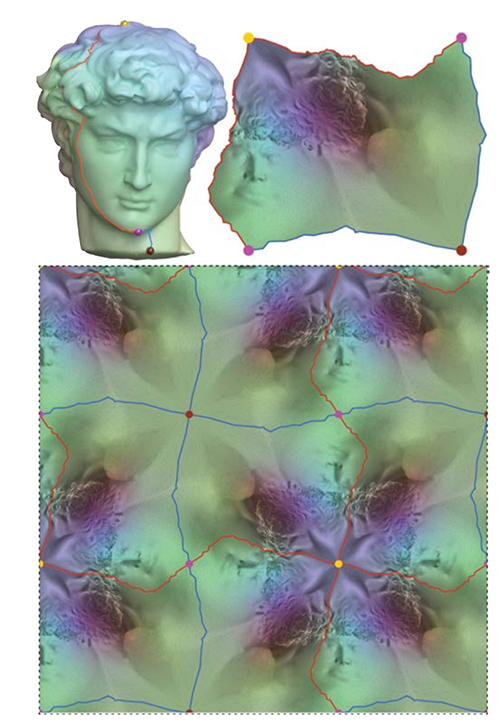
\includegraphics[width=0.3\textwidth]{images/tiles.png}
    \caption{An example of tiling of $\mathbb{R}^2$}
    \label{Fig:tiles}
    \end{figure}
    
    
    \begin{figure}
    \centering
  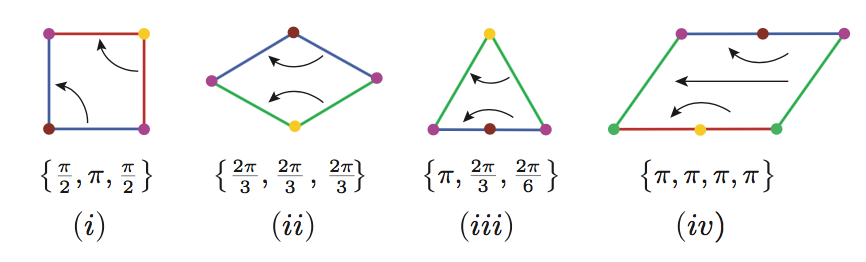
\includegraphics[width=0.4\textwidth]{images/orbifolds}
    \caption{4 kinds of 2-dimension Euclidean orbifolds.}
    \label{Fig:orbifolds}
    \end{figure}
    Injective parameterizations of surface meshes are vital for many applications in Computer Graphics, Geometry Processing and related fields. Only a few algorithms are guaranteed to produce injective parameterizations that are also globally optimal in some well-defined sense. The main approach known to provide such a guarantee is Tutte’s embedding and its generalization to convex combination maps (CCM). However, CCM is currently limited to injective parameterizations of disk-type and toric surfaces, leaving the arguably most common case of spherical surfaces untreated. And this paper is to handle this problem.
    
    This paper proposed the orbifold-Tutte planar embedding. It is a generalization of Tutte’s embedding and CCM to other topologies. It can bijectively maps the original surface to a canonical, topologically equivalent, two-dimensional flat surface with cone singularities, called a Euclidean orbifold.
    
    Orbifold is a generalization of the concept of manifold. Manifolds are locally euclidean, and orbifolds are locally euclidean under some group. There are 17 2-dimensional Euclidean orbifolds in total, which are corresponding to 17 wall paper groups. These orbifolds can be treated as the quotient space of $\mathbb{R}^2$ by some paper group. So $\mathbb{R}^2$ can be tiled seamlessly with the base domain of these orbifolds (i.e. Fig. \ref{Fig:tiles}). This is the key point in proving the injectiveness of orbifold Tutte embedding.
    
    Out of all Euclidean orbifold, four of them have spherical topology (Fig. \ref{Fig:orbifolds}). This project will use these four orbifolds to achieve flat embedding of sphere-type surface.
    
    The pipline of embedding can be summarized as follows:
    \begin{enumerate}
    \item Choose some cone vertices and slice through them to get a disk-type surface.
    \item Solve a sparse linear system to get the global injective map from sliced surface to $\mathbb{R}^2$ which realizes the bijective map from original surface to its corresponding orbifold.
    \end{enumerate}
  	
   
    
% Main Part
\section{Weekly Plan}
	% LaTeX takes complete care of your document layout ...
	This project will reimplement the algorithm method of this paper and apply it to texture mapping. 
    I will separate the whole software system into three components: view port with texture mapping function, mesh operations (for example, slice the mesh) and the sparse linear system solver. The weekly plan is as follows:
   \begin{enumerate}
   \item By week 2: Read the paper carefully to figure out the details of the background theory and the algorithm.
   \item By week 4: Build a UI system which can show surface mesh and its texture.
   \item By week 6: Implemented all mesh operations that the algorithm needed, including slicing the mesh along a line. 
   \item By week 8: Build the sparse solver for the algorithm.
   \item By week 10: Test and improve the whole system.
   \end{enumerate}
If time is enough, I'll also implement the algorithms in \cite{aigerman2016hyperbolic} and \cite{aigerman2017spherical}. They applied orbifold to different background geometries.

% Now we need a bibliography:
\begin{thebibliography}{5}

	%Each item starts with a \bibitem{reference} command and the details thereafter.
    \bibitem{aigerman2015orbifold}
    Aigerman, N., \& Lipman, Y. (2015). Orbifold Tutte Embeddings. ACM Transactions on Graphics (TOG) - Proceedings of ACM SIGGRAPH Asia 2015, 34(6). 
    \bibitem{aigerman2016hyperbolic}
    Aigerman, N., \& Lipman, Y. (2016). Hyperbolic orbifold tutte embeddings. ACM Transactions on Graphics (TOG) - Proceedings of ACM SIGGRAPH Asia 2016, 35(6). 

\bibitem{aigerman2017spherical}
Aigerman, N., Kovalsky, S. Z., \& Lipman, Y. (2017). Spherical Orbifold Tutte Embeddings. ACM Transactions on Graphics (TOG), 36(4). 


\end{thebibliography}

% Your document ends here!
\end{document}